\providecommand{\PATH}{.}%\PATH=.と置く
%https://tex.stackexchange.com/questions/289450/path-of-figures-in-different-directories-with-subfile-latex
%----以下文字の大きさ,フォント,余白などを決定する設定----
\documentclass[a4paper,10pt]{jsarticle}
\bibliographystyle{junsrt} %参考文献の並べ順junsrtの場合,本文内で参照した順
\setlength{\topmargin}{-17truemm}
\setlength{\oddsidemargin}{-0.4truemm}
\setlength{\textwidth}{160truemm}
\setlength{\textheight}{247truemm}
%-------------------------------------------------
%コンパイル方法 platex hoge.tex → platex hoge.tex → dvipdfmx hoge(サブファイルでも実行可能※ただし,サブファイルでコンパイルすると「他のサブファイルで定義された」ラベルを参照した時に?になる)
%bibtex適用のコンパイル platex hoge.tex → pbibtex hoge.tex → platex hoge.tex → platex hoge.tex → dvipdfmx hoge(メインファイルでのみ実行可能※サブファイルではコンパイルエラーが起きる)
%\usepackage{}:Latexで拡張機能を使用するための宣言-------------
\usepackage[dvipdfmx]{graphicx}%図を埋め込むためのパッケージ
\usepackage{longtable}%ページをまたぐ表を表示させるパッケージ
\usepackage{float}%その場に表・図を表示させるパッケージ
\usepackage{listings,jlisting}%ソースコードを埋め込むためのパッケージ(jlistingはサイトからDLする必要あり)
%Windowsにjlistingパッケージを導入する https://mildtech.hatenablog.com/entry/2017/07/24/160324
\usepackage[dvipdfmx]{hyperref}%しおり作成のためのパッケージ
\usepackage{pxjahyper}%しおりを日本語化
\usepackage{amsmath}%数式関連のパッケージ(alignなど)
\usepackage{bm}%太字でベクトルを表記
\usepackage{subfiles}%サブファイル
\usepackage{tabularx}%表内セルを良いところで改行
\usepackage[linesnumbered,ruled,lined, noend]{algorithm2e} %アルゴリズムを記述(外部パッケージ:https://www.ctan.org/pkg/algorithm2e)

% ---- new command (標準でコマンドがない記述形式をコマンド化)-----------------
\newcommand{\ita}[1]{\textit{#1}}%イタリック体太字
\newcommand{\rma}[1]{\textrm{#1}}%ローマン体
\newcommand{\bdit}[1]{\textit{\textbf{#1}}}%イタリック体太字
\newcommand{\bdrm}[1]{\textrm{\textbf{#1}}}%ローマン体太字
\newcommand{\argmin}{\mathop{\rm arg~min}\limits}%arg min
\newcommand{\argmax}{\mathop{\rm arg~max}\limits}%arg max
%------------------------------------------------------------------

\lstset{%ソースコードを書き込む時の設定--------------------------------
  language=C++,%言語
  columns=[l]{fullflexible}, % 文字をつめる
  basicstyle=\footnotesize,%
  commentstyle=\textit,%
  classoffset=1,%
  keywordstyle=\bfseries,%
	frame=tRBl,framesep=5pt,%枠線の種類 frame=singleならば一重枠
  showstringspaces=false,%
  numbers=left,stepnumber=1,numberstyle=\footnotesize,%
  breaklines=true,%trueで1行が長い時に改行
  firstnumber=1,%行番号が何番から始まるか
  xrightmargin=1zw,%枠右側の余白
  xleftmargin=1zw%枠左側の余白
}%本文中に \lstinputlisting[caption=キャプション,label=ラベル]{ファイル名}でソースコードを貼り付け
%--------------------------------------------------------------------

\title{タイトル}%タイトル
\author{田中太郎}%著者
\date{2000年1月1日}%日付

\begin{document}%本文の始まり
\maketitle%上記で設定したtitle,author,dateを表示

%subfile
\subfile{subfile/subfile.tex}

\section{文字(newcommand)}
newcommandで新しく定義したコマンドを使用して記述する.
イタリック体\ita{italic}で記述する.\\
ローマン体\rma{roman}で記述する.\\
イタリック体太字\bdit{bditalic}で記述する.\\
ローマン体太字\bdrm{bdrma}で記述する.
arg\_minとarg\_maxを記述する.
$$ \argmin_{\bdrm{x}}$$
$$ \argmax_{\bdrm{x}}$$


\section{式}
式(\ref{eq:hoge})を参照する.
\begin{gather}
    x_{1}=L_{1} \cos \theta_{1}
    \label{eq:hoge}
\end{gather}

\section{図}
図\ref{fig:hoge}を参照する.
\begin{figure}[H]
    \begin{center}
        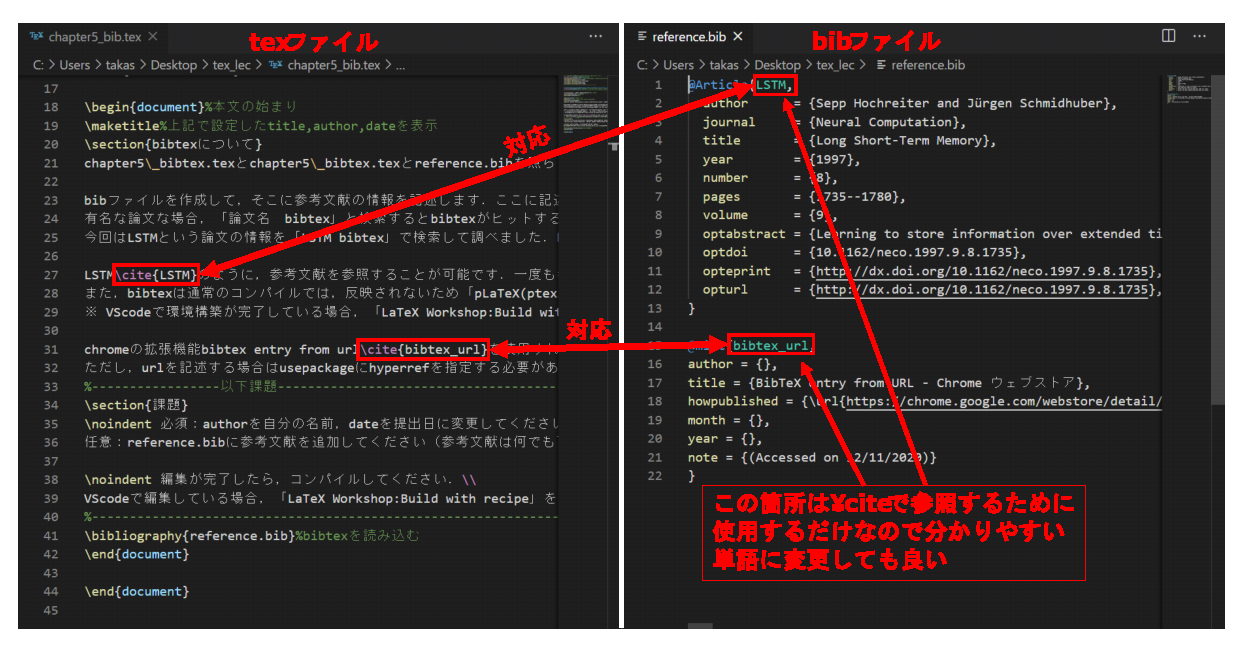
\includegraphics[width=120mm]{\PATH/fig/bibtex.eps}
    \end{center}
    \caption{hoge}
    \label{fig:hoge}
\end{figure}

\section{表}
表\ref{tb:hoge}を参照する.
\begin{table}[H]
    \caption{hoge}
    \label{tb:hoge}
    \centering
    \begin{tabular}{ll}
        \hline
        title1 & title2 \\
        \hline \hline
        hoge1 & hoge2 \\
        \hline
    \end{tabular}
\end{table}

\section{コード}
コード\ref{code:hoge}を参照する.
\lstinputlisting[language=python, caption = title, label = code:hoge]{code/code.py}

\section{注釈}
論文以外の参照(URLなど)は注釈\footnote{\url{https://github.com/ros-simulation/gazebo_ros_demos}}を使うことがある.



\section{アルゴリズム}
{\bf{Algorithm}} \ref{alg:hoge}に示す.

\begin{algorithm*}[H]
    \small{
        \caption{title}
        \label{alg:hoge}
        \For{$i=1, \cdots, n $}
        {
            \If{$i == 5$}
            {
                OK;
            }
            \Else
            {
                No;
            }
        }
        \Return A
    }
\end{algorithm*}

\section{参考文献を参照}
PointNet\cite{point_net}を参照する.

%参考文献(bibtex(参考文献を反映させるときはpbibtexコマンドを使用
% \nocite{*} %http://regry358.hatenablog.com/entry/2014/10/16/140251 参照していない文献も表示
\bibliographystyle{jIEEEtran.bst}
\bibliography{reference.bib}
% https://github.com/ehki/jIEEEtran
% IEEJtran.bst : 電気学会の日英両対応版
% jIEEJtran.bst : IEEEtranの日本語対応版
% mixej.py : 同一文献で日本語と英語を併記するためのスクリプト

\end{document}

%-------ラベル,参照----------
%\label{sec:hoge}
%\label{fig:hoge}
%\label{eq:hoge}
%\ref{sec:hoge}

%公式------------------
%\begin{gather}
%    x_{1}=L_{1} \cos \theta_{1}
%    \label{eq:hoge}
%\end{gather}

%式--------------------
%$x_1$

%図--------------------
%\begin{figure}[H]
%    \begin{center}
%        \includegraphics[width=120mm]{\PATH/fig/hoge.eps}
%    \end{center}
%    \caption{hoge}
%    \label{fig:hoge}
%\end{figure}

%表-------------------------
%\begin{table}[H]
%    \caption{hoge}
%    \label{tb:hoge}
%    \centering
%    \begin{tabular}{ll}
%        \hline
%        title1 & title2 \\
%        \hline \hline
%        hoge1 & hoge2 \\
%        \hline
%    \end{tabular}
%\end{table}

%下記は表の内容が長すぎた場合,いいところで改行してくれる
%\begin{table}[H]
%    \caption{hoge}
%    \label{tb:hoge}
%    \centering
%    \begin{tabularx}{\linewidth}{lX}
%        \hline
%        title1 & title2 \\
%        \hline \hline
%        hoge1 & hoge2 \\
%        \hline
%    \end{tabularx}
%\end{table}

% ------- ソースコード -------------------
% \lstinputlisting[language=python, caption = title, label = code:hoge]{code/code.py}

%参考文献,サイトの参照-----
%\cite{motion-planning}

%特殊文字--------------------
%http://www.ic.daito.ac.jp/~mizutani/tex/special_characters.html

%注意点-------------------------------
%式を参照する時は「式(\ref{eq:hoge})」のように()で囲む
%式,図,表,参考文献の全てにおいてレポート内で一度は参照する
%正式名称が存在する単語は「Rapidly-exploring random tree(RRT)」のように,最初の一度のみ正式名称を記す(2回目以降は略称でも可)
%表,図のタイトルの最後にはピリオド(.)をつける
